\documentclass[border=10pt]{standalone}
\usepackage[svgnames]{xcolor}
\usepackage{amsmath}
\usepackage{pgfplots}
\pgfplotsset{compat=newest}
\usepackage[sfdefault]{FiraSans}
\usepackage{FiraMono}
\renewcommand*\familydefault{\sfdefault}
\begin{document}
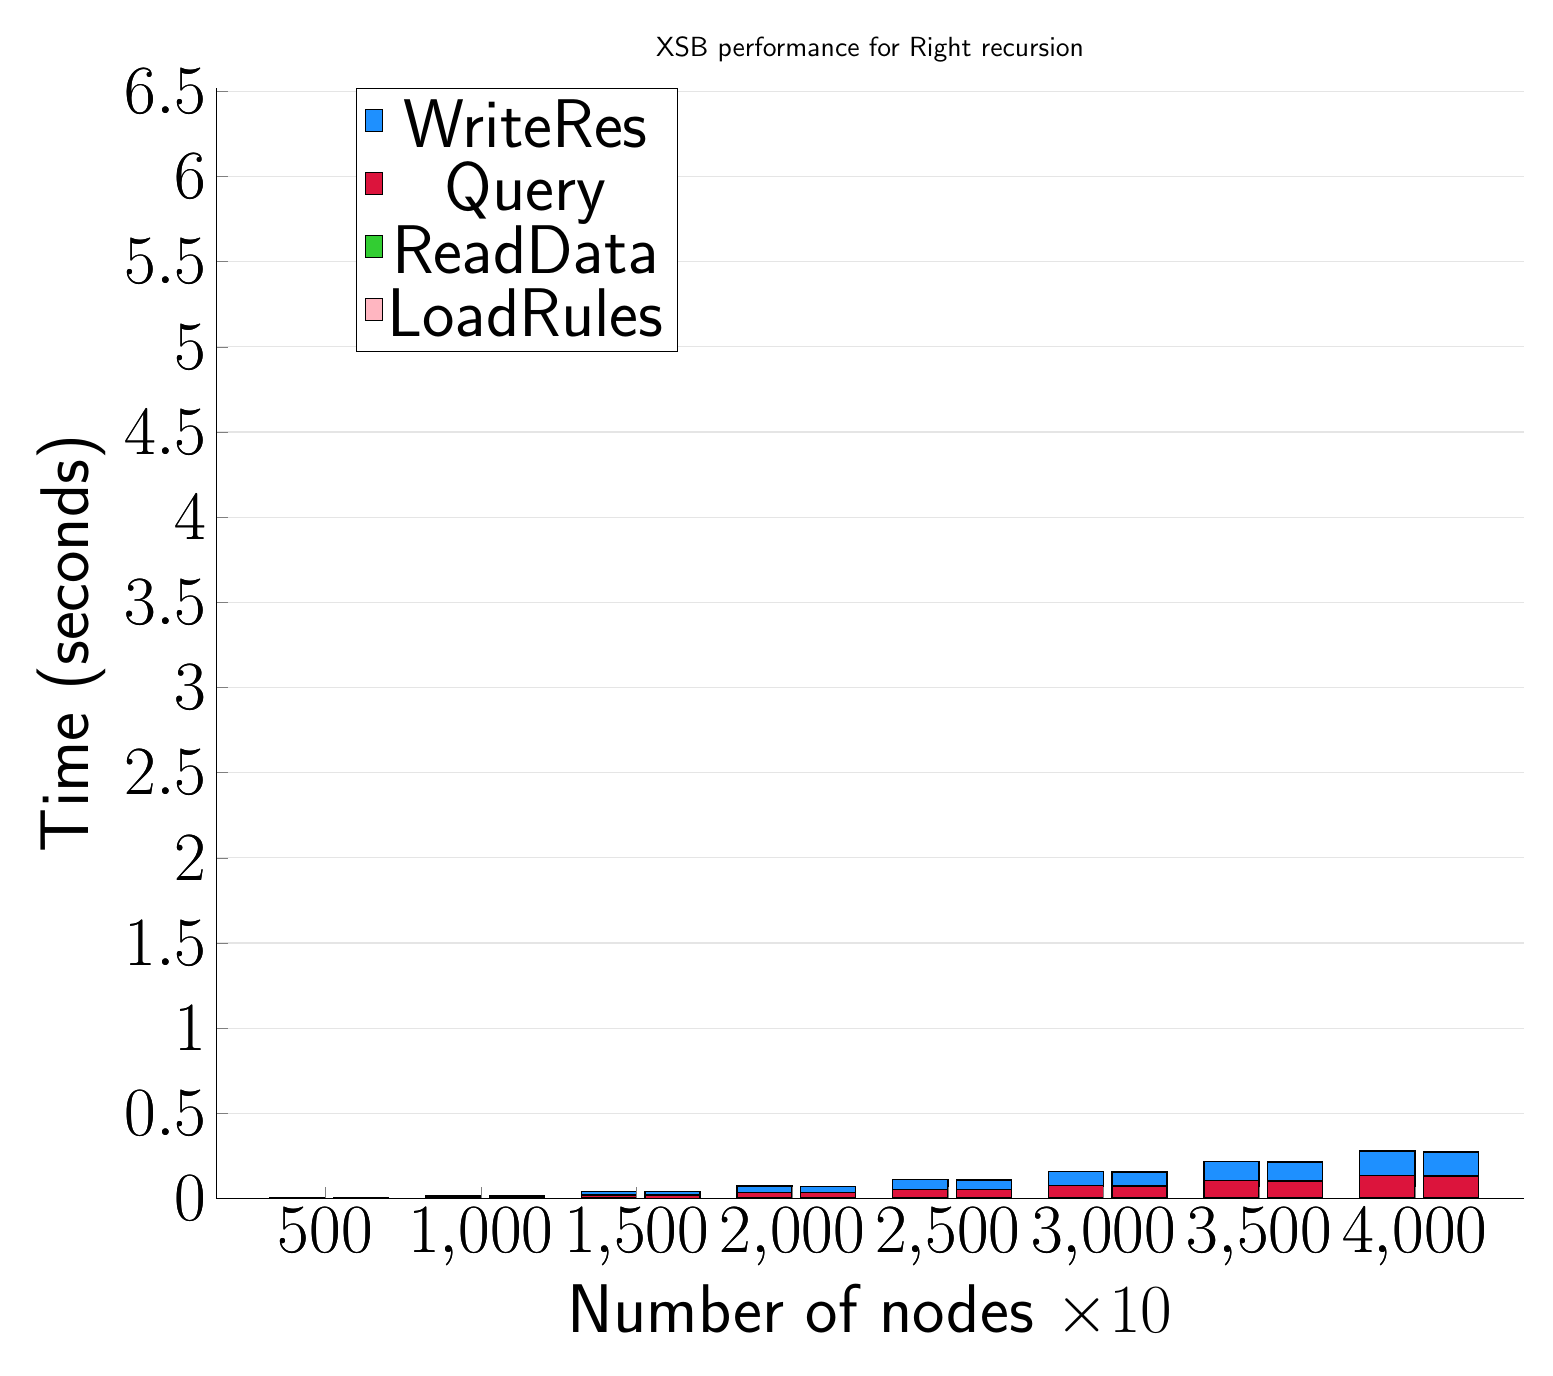
\begin{tikzpicture}
\begin{axis}[
   ybar stacked,
   title={XSB performance for Right recursion},
   bar shift=-10pt,
   width=1.5\textwidth,
   bar width=0.7cm,
   ymajorgrids, tick align=inside,
   major grid style={draw=gray!20},
   xtick=data,
   ymin=0, ymax=6.52002317905426,
   axis x line*=bottom,
   axis y line*=left,
   enlarge x limits=0.1,
   legend style={
       at={(0.23, 1)},
       anchor=north,
       legend columns=1,
       font=\Huge,
   },
   ylabel={Time (seconds)},
   xlabel={Number of nodes $\times 10$},
   label style={font=\Huge},
   tick label style={font=\Huge},
]
\addlegendimage{fill=DodgerBlue, draw=black, line width=0.2pt}
\addlegendentry{WriteRes}
\addlegendimage{fill=Crimson, draw=black, line width=0.2pt}
\addlegendentry{Query}
\addlegendimage{fill=LimeGreen, draw=black, line width=0.2pt}
\addlegendentry{ReadData}
\addlegendimage{fill=LightPink, draw=black, line width=0.2pt}
\addlegendentry{LoadRules}
\addplot +[fill=LightPink, draw=black, line width=0.5pt] coordinates {
    (500, 0.0010905504226684571)
    (1000, 0.001076197624206544)
    (1500, 0.001031589508056639)
    (2000, 0.001084947586059571)
    (2500, 0.001068377494812011)
    (3000, 0.001075506210327148)
    (3500, 0.0010982990264892583)
    (4000, 0.0010788440704345712)
};
\addplot +[fill=LimeGreen, draw=black, line width=0.5pt] coordinates {
    (500, 0.0008495807647705078)
    (1000, 0.001374626159667968)
    (1500, 0.0019435882568359386)
    (2000, 0.0024827241897583006)
    (2500, 0.0030372858047485354)
    (3000, 0.0035847902297973635)
    (3500, 0.004074716567993164)
    (4000, 0.004602003097534179)
};
\addplot +[fill=Crimson, draw=black, line width=0.5pt] coordinates {
    (500, 0.0018490791320800789)
    (1000, 0.0076640605926513675)
    (1500, 0.018208813667297364)
    (2000, 0.03187992572784423)
    (2500, 0.04927480220794677)
    (3000, 0.07238552570343017)
    (3500, 0.09944252967834474)
    (4000, 0.13074789047241211)
};
\addplot +[fill=DodgerBlue, draw=black, line width=0.5pt] coordinates {
    (500, 0.0025157451629638653)
    (1000, 0.009700512886047364)
    (1500, 0.021657919883728026)
    (2000, 0.03788444995880128)
    (2500, 0.058705282211303736)
    (3000, 0.08244328498840334)
    (3500, 0.11425819396972645)
    (4000, 0.1427615165710451)
};
\end{axis}
\begin{axis}[
   ybar stacked,
   bar shift=13pt,
   width=1.5\textwidth,
   bar width=0.7cm,
   ymajorgrids, tick align=inside,
   major grid style={draw=none},
   xtick=data,
   ymin=0, ymax=6.52002317905426,
   axis x line*=none,
   axis y line*=none,
   enlarge x limits=0.1,
   label style={font=\Huge},
   tick label style={font=\Huge},
]
\addplot +[fill=LightPink, draw=black, line width=0.5pt] coordinates {
    (500, 0.0006253)
    (1000, 0.0006136)
    (1500, 0.0006001000000000002)
    (2000, 0.000606)
    (2500, 0.0006076000000000001)
    (3000, 0.0006142999999999999)
    (3500, 0.0006074000000000003)
    (4000, 0.0006166999999999996)
};
\addplot +[fill=LimeGreen, draw=black, line width=0.5pt] coordinates {
    (500, 0.0006023999999999995)
    (1000, 0.0010711)
    (1500, 0.0015419000000000001)
    (2000, 0.0020320999999999994)
    (2500, 0.0025322000000000005)
    (3000, 0.0030338000000000006)
    (3500, 0.003508700000000001)
    (4000, 0.0039737999999999996)
};
\addplot +[fill=Crimson, draw=black, line width=0.5pt] coordinates {
    (500, 0.0018156)
    (1000, 0.007549499999999999)
    (1500, 0.0179535)
    (2000, 0.03140049999999999)
    (2500, 0.048666)
    (3000, 0.0712826)
    (3500, 0.0981746)
    (4000, 0.1285222)
};
\addplot +[fill=DodgerBlue, draw=black, line width=0.5pt] coordinates {
    (500, 0.0022570000000000003)
    (1000, 0.009241200000000001)
    (1500, 0.0205551)
    (2000, 0.036341500000000006)
    (2500, 0.05707829999999999)
    (3000, 0.0808805)
    (3500, 0.1121383)
    (4000, 0.14042190000000002)
};
\end{axis}
\end{tikzpicture}

\end{document}
